\documentclass[tikz,border=25pt]{standalone}
\usepackage{amsmath, amssymb}
\usetikzlibrary{matrix, positioning, fit, backgrounds, calc}

\begin{document}
	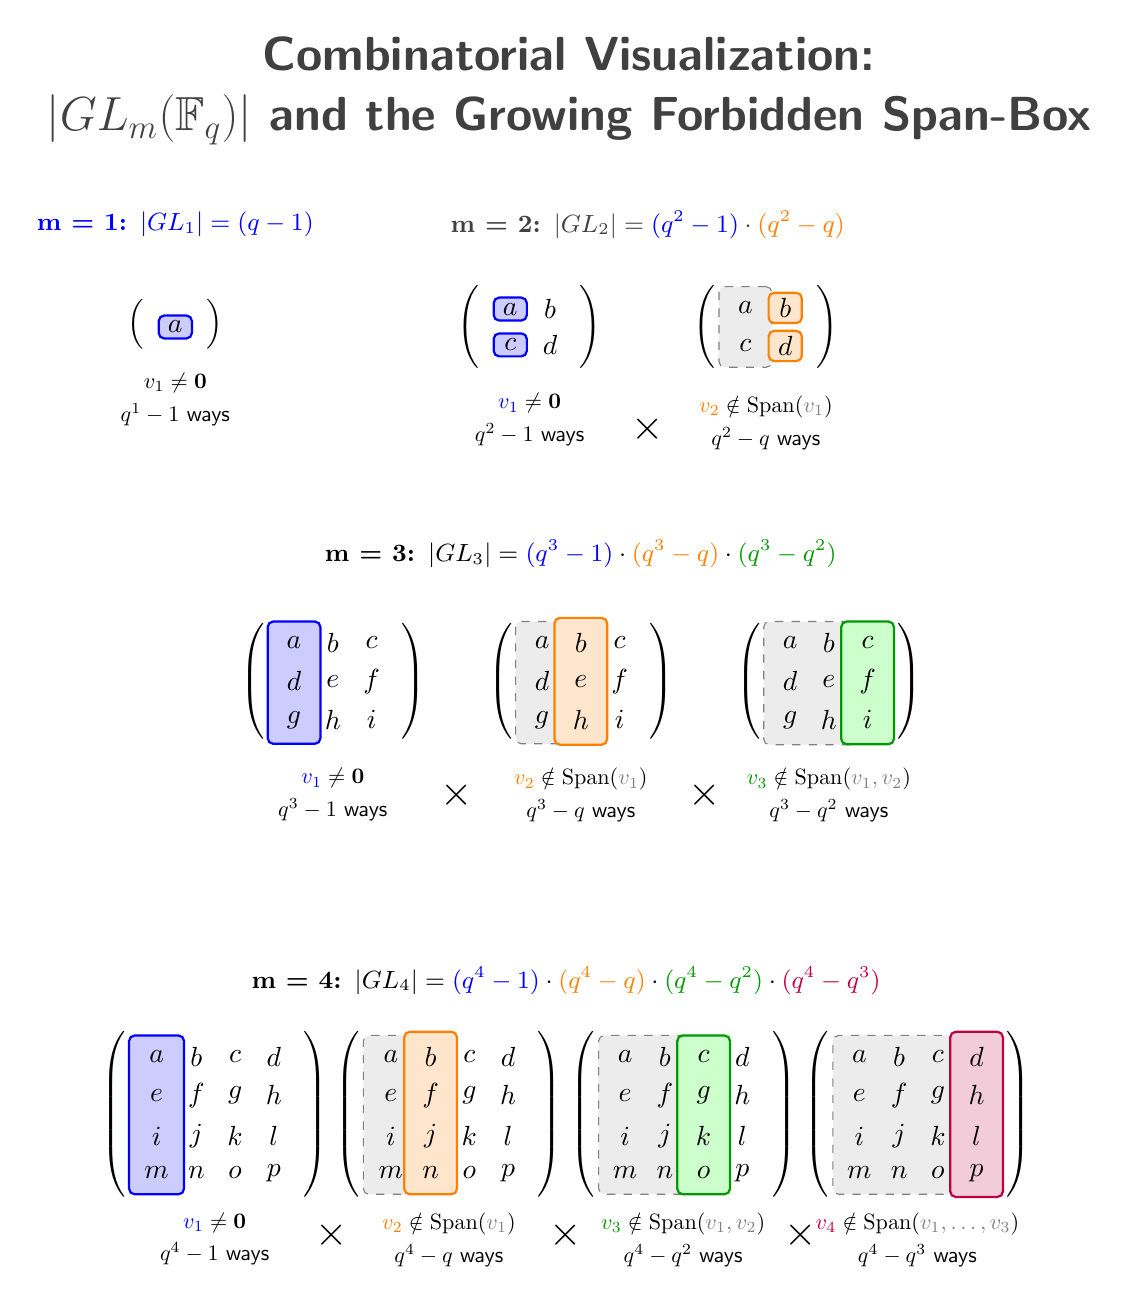
\begin{tikzpicture}[
		font=\sffamily,
		% Style for the matrices
		mtx/.style={
			matrix of math nodes,
			left delimiter=(, right delimiter=),
			nodes={minimum width=1.2em, inner sep=2pt, anchor=center},
			column sep=2pt, row sep=2pt,
			ampersand replacement=\&
		},
		% Highlighting styles for active columns
		hl-v1/.style={fill=blue!20, draw=blue, thick, rounded corners=2pt},
		hl-v2/.style={fill=orange!20, draw=orange, thick, rounded corners=2pt},
		hl-v3/.style={fill=green!20, draw=green!60!black, thick, rounded corners=2pt},
		hl-v4/.style={fill=purple!20, draw=purple, thick, rounded corners=2pt},
		% Style for the accumulating "Span Box"
		hl-span/.style={fill=gray!15, draw=gray, dashed, rounded corners=2pt},
		% Title & Text
		mainTitle/.style={font=\sffamily\bfseries\LARGE, color=darkgray, align=center},
		term label/.style={font=\bfseries\small, align=center}
		]
		
		% ==============================================================================
		% MAIN TITLE
		% ==============================================================================
		\node[mainTitle] (title) at (0, 7.5) {Combinatorial Visualization:\\$|GL_m(\mathbb{F}_q)|$ and the Growing Forbidden Span-Box};
		
		% ==============================================================================
		% ROW 1: m = 1 and m = 2 (Small Cases)
		% ==============================================================================
		
		% CASE m = 1
		\begin{scope}[shift={(-5, 4.5)}, scale=1]
			\node[term label, text=blue] at (0, 1.3) {m = 1: $|GL_1| = \textcolor{blue}{(q-1)}$};
			\matrix[mtx] (M1) at (0, 0) {
				|[hl-v1]| a \\
			};
			\node[below=0.2cm of M1, align=center, scale=0.8] {
				$v_1 \neq \mathbf{0}$ \\[1mm]
				\textbf{$q^1 - 1$} ways
			};
		\end{scope}
		
		% CASE m = 2
		\begin{scope}[shift={(1, 4.5)}, scale=1]
			\node[term label, text=darkgray] at (0, 1.3) {m = 2: $|GL_2| = \textcolor{blue}{(q^2-1)} \cdot \textcolor{orange}{(q^2-q)}$};
			\matrix[mtx] (M2_1) at (-1.5, 0) {
				|[hl-v1]| a \& b \\
				|[hl-v1]| c \& d \\
			};
			\matrix[mtx] (M2_2) at (1.5, 0) {
				a \& |[hl-v2]| b \\
				c \& |[hl-v2]| d \\
			};
			\begin{scope}[on background layer]
				\node[hl-span, fit=(M2_2-1-1)(M2_2-2-1)] {}; % v1 is forbidden
			\end{scope}
			
			\node[below=0.2cm of M2_1, align=center, scale=0.8] {
				$\textcolor{blue}{v_1} \neq \mathbf{0}$ \\[1mm]
				\textbf{$q^2 - 1$} ways
			};
			\node[below=0.2cm of M2_2, align=center, scale=0.8] {
				$\textcolor{orange}{v_2} \notin \mathrm{Span}(\textcolor{gray}{v_1})$ \\[1mm]
				\textbf{$q^2 - q$} ways
			};
			
			% Draw multiplication sign after both nodes exist
			\node[scale=1.5] at ($(M2_1)!0.5!(M2_2)+(0,-1.3)$) {$\times$};
		\end{scope}
		
		% ==============================================================================
		% ROW 2: m = 3 (Scaling Up)
		% ==============================================================================
		\begin{scope}[shift={(-3, 0)}, scale=0.9]
			\node[term label] at (3.5, 1.8) {m = 3: $|GL_3| = \textcolor{blue}{(q^3-1)} \cdot \textcolor{orange}{(q^3-q)} \cdot \textcolor{green!60!black}{(q^3-q^2)}$};
			
			% Column 1
			\matrix[mtx] (M3_1) at (0, 0) {
				a \& b \& c \\
				d \& e \& f \\
				g \& h \& i \\
			};
			\begin{scope}[on background layer] \node[hl-v1, fit=(M3_1-1-1)(M3_1-3-1)] {}; \end{scope}
			\node[below=0.2cm of M3_1, align=center, scale=0.8] {
				$\textcolor{blue}{v_1} \neq \mathbf{0}$ \\[1mm]
				\textbf{$q^3 - 1$} ways
			};
			
			% Column 2
			\matrix[mtx] (M3_2) at (3.5, 0) {
				a \& b \& c \\
				d \& e \& f \\
				g \& h \& i \\
			};
			\begin{scope}[on background layer]
				\node[hl-span, fit=(M3_2-1-1)(M3_2-3-1)] {}; % v1 forbidden
				\node[hl-v2, fit=(M3_2-1-2)(M3_2-3-2)] {};
			\end{scope}
			\node[below=0.2cm of M3_2, align=center, scale=0.8] {
				$\textcolor{orange}{v_2} \notin \mathrm{Span}(\textcolor{gray}{v_1})$ \\[1mm]
				\textbf{$q^3 - q$} ways
			};
			
			% Column 3
			\matrix[mtx] (M3_3) at (7, 0) {
				a \& b \& c \\
				d \& e \& f \\
				g \& h \& i \\
			};
			\begin{scope}[on background layer]
				\node[hl-span, fit=(M3_3-1-1)(M3_3-3-2)] {}; % v1, v2 forbidden
				\node[hl-v3, fit=(M3_3-1-3)(M3_3-3-3)] {};
			\end{scope}
			\node[below=0.2cm of M3_3, align=center, scale=0.8] {
				$\textcolor{green!60!black}{v_3} \notin \mathrm{Span}(\textcolor{gray}{v_1, v_2})$ \\[1mm]
				\textbf{$q^3 - q^2$} ways
			};
			
			% Draw multiplication signs after nodes exist
			\node[scale=1.5] at ($(M3_1)!0.5!(M3_2)+(0,-1.6)$) {$\times$};
			\node[scale=1.5] at ($(M3_2)!0.5!(M3_3)+(0,-1.6)$) {$\times$};
		\end{scope}
		
		% ==============================================================================
		% ROW 3: m = 4 (Generalizing)
		% ==============================================================================
		\begin{scope}[shift={(-4.5, -5.5)}, scale=0.85]
			\node[term label] at (5.25, 2.0) {m = 4: $|GL_4| = \textcolor{blue}{(q^4-1)} \cdot \textcolor{orange}{(q^4-q)} \cdot \textcolor{green!60!black}{(q^4-q^2)} \cdot \textcolor{purple}{(q^4-q^3)}$};
			
			% Col 1
			\matrix[mtx] (M4_1) at (0, 0) {
				a \& b \& c \& d \\
				e \& f \& g \& h \\
				i \& j \& k \& l \\
				m \& n \& o \& p \\
			}; 
			\begin{scope}[on background layer] \node[hl-v1, fit=(M4_1-1-1)(M4_1-4-1)] {}; \end{scope}
			\node[below=0.1cm of M4_1, align=center, scale=0.8] {
				$\textcolor{blue}{v_1} \neq \mathbf{0}$ \\[1mm]
				\textbf{$q^4 - 1$} ways
			};
			
			% Col 2
			\matrix[mtx] (M4_2) at (3.5, 0) {
				a \& b \& c \& d \\
				e \& f \& g \& h \\
				i \& j \& k \& l \\
				m \& n \& o \& p \\
			};
			\begin{scope}[on background layer]
				\node[hl-span, fit=(M4_2-1-1)(M4_2-4-1)] {};
				\node[hl-v2, fit=(M4_2-1-2)(M4_2-4-2)] {};
			\end{scope}
			\node[below=0.1cm of M4_2, align=center, scale=0.8] {
				$\textcolor{orange}{v_2} \notin \mathrm{Span}(\textcolor{gray}{v_1})$ \\[1mm]
				\textbf{$q^4 - q$} ways
			};
			
			% Col 3
			\matrix[mtx] (M4_3) at (7.0, 0) {
				a \& b \& c \& d \\
				e \& f \& g \& h \\
				i \& j \& k \& l \\
				m \& n \& o \& p \\
			};
			\begin{scope}[on background layer]
				\node[hl-span, fit=(M4_3-1-1)(M4_3-4-2)] {};
				\node[hl-v3, fit=(M4_3-1-3)(M4_3-4-3)] {};
			\end{scope}
			\node[below=0.1cm of M4_3, align=center, scale=0.8] {
				$\textcolor{green!60!black}{v_3} \notin \mathrm{Span}(\textcolor{gray}{v_1, v_2})$ \\[1mm]
				\textbf{$q^4 - q^2$} ways
			};
			
			% Col 4
			\matrix[mtx] (M4_4) at (10.5, 0) {
				a \& b \& c \& d \\
				e \& f \& g \& h \\
				i \& j \& k \& l \\
				m \& n \& o \& p \\
			};
			\begin{scope}[on background layer]
				\node[hl-span, fit=(M4_4-1-1)(M4_4-4-3)] {};
				\node[hl-v4, fit=(M4_4-1-4)(M4_4-4-4)] {};
			\end{scope}
			\node[below=0.1cm of M4_4, align=center, scale=0.8] {
				$\textcolor{purple}{v_4} \notin \mathrm{Span}(\textcolor{gray}{v_1, \dots, v_3})$ \\[1mm]
				\textbf{$q^4 - q^3$} ways
			};
			
			% Draw multiplication signs after nodes exist
			\node[scale=1.5] at ($(M4_1)!0.5!(M4_2)+(0,-1.8)$) {$\times$};
			\node[scale=1.5] at ($(M4_2)!0.5!(M4_3)+(0,-1.8)$) {$\times$};
			\node[scale=1.5] at ($(M4_3)!0.5!(M4_4)+(0,-1.8)$) {$\times$};
		\end{scope}
		
	\end{tikzpicture}
\end{document}